\chapter{A Framework for SV Detection in MapReduce}\label{chap_framework}

\section{MapReduce and Hadoop}\label{section_hadoop_description}

MapReduce~\cite{Dean:2008p277} divides computation across a cluster into three phases. In the first phase, \emph{mappers} developed by the application programmer examine small blocks of data and emit a set of $\langle key, value \rangle$ pairs for each block examined. The MapReduce framework then sorts the output of the mappers by key, and aggregates all values that are associated with each key. Finally, the framework executes \emph{reducers}, also created by the application developer, which process all of the values for a particular key and produce one or more outputs that summarize or aggregate those values. MapReduce and Hadoop allow efficient processing of large data sets by scheduling tasks for execution as close as possible to the nodes which hold the required data, minimizing network traffic and I/O contention.

\section{Uses of Hadoop and MapReduce in Sequencing Tasks}

The Hadoop framework has been used for a variety of sequencing-related bioinformatic tasks. Figure~\ref{bio_hadoop_ecosystem} gives an overview of the published applications of Hadoop to three popular sequencing pipelines: DNA resequencing, RNA-seq, and \emph{de novo} assembly. In some cases, researchers have developed native MapReduce algorithms to solve particular problems. In other instances, Hadoop has been used to run existing tools in parallel; of course, this is only possible when the tasks are embarassingly parallel at some level. Finally, there are several lower-level APIs, toolkits, and frameworks that have been created in an attempt to ease the development of Hadoop pipelines. These toolkits provide wrappers for reading and writing popular sequencing related file formats, wrappers for commonly used tools, and functions to manipulate short read sequences and alignment records. We will discuss each of these pipelines in more detail in the following sections.

\begin{figure}
\centering

\includegraphics[width=1\textwidth]{figures/bio_hadoop_ecosystem.pdf}
\caption{Hadoop applications to tasks of three popular sequencing analysis pipelines. Solid lines indicate native MapReduce applications developed specifically for Hadoop. Dotted lines indicate pipelines that parallelize the execution of existing tools on splits of the input data using Hadoop. In addition, several toolkits and frameworks are listed that are broadly applicable to many portions of these pipelines.}
\label{bio_hadoop_ecosystem}
\end{figure}

\subsection{DNA Resequencing}

As we discussed in Section~\ref{section_pipelines}, there are multiple steps that are typically part of DNA resequencing pipelines. These steps included quality control analysis, alignment to the genome reference, a series of processes including realignment in problematic regions and removal of duplicate reads, steps to call SNVs and SVs, and finally annotation and analysis of the variants that were discovered. 

A native algorithm for mapping short reads to a reference genome was first demonstrated in Cloudburst~\cite{Schatz:2009p278}. This algorithm creates keys for each k-mer that appears in both the reads and the reference. The reducers then bring together the reads and portions of the reference that match on the same k-mer, and determine whther the match on the seed can be extended to an alignment of the entire read to the reference. Because the read and reference portions are each transfered to the reducers for every single k-mer which appears in them, this algorithm, while accurate, generates large amounts of data that must be shuffled, sorted, and potentially cross the network. Therefore, it is difficult to scale it to very large read sets. This shows the difficulty of designing true MapReduce algorithms that can scale and take advantages of Hadoop's infrastructure. CloudAligner~\cite{Nguyen:2011p1832} uses a similar seed-and-extend algorithm, although the exact details of their map and reduce steps are not specified.

Since short read mapping is an embarrassingly parallel task and highly optimized non-MapReduce alignment tools with full feature sets are readily available, it is more efficient in practice to use the map phase of a Hadoop job to align splits of input reads with existing tools, and then merge results in the reduce phase. SEAL~\cite{Pireddu:2011fj} and the CRS4 Sequencing and Genotyping Platform's CSGP workflow~\cite{Pireddu:2011:MGS:1996092.1996106} are two such pipelines which use the BWA~\cite{Li:2009p836} aligner in each map task. By emitting mappings under a key for the alignment location, they are then able to accomplish the duplicate removal step in the reduce function in a manner similar to that of the popular non-MapReduce tool Picard~\cite{picard}. Similarly, Crossbow~\cite{Langmead:2009p1225} uses Hadoop to parallelize Bowtie~\cite{Langmead:2009p768}. Crossbow then calls single nucleotide variants in the reduce phase using SOAPsnp~\cite{Li:2009p1236}, allowing it to function as a minimum viable pipeline for sequencing. Crossbow also includes infrastructure for running in the Amazon Elastic Compute Cloud, which has contributed to its popularity. SeqInCloud~\cite{nabeel-bicob13-genome-analysis-cloud} similarly combines BWA with the GATK's~\cite{McKenna:2010p1051} realignment and SNV calling steps, along with infrastrucure to run in the Microsoft Azure cloud computing platform.

After variant discovery, the usual next step in a resequencing project is to analyze the variants found to detect functional impact (i.e. what genes might be disrupted by the variants found) or to find associations between variants and phenotypes, as in case-control sequencing projects. SeqWare~\cite{Oconnor:2010p1835} uses HBase~\cite{hbase}, a Hadoop database based upon Google's BigTable~\cite{Chang:2008:BDS:1365815.1365816}, to provide functionality to annotate and query the variants. SeqWare uses the genomic coordinates of variants and coverage information as schema keys within HBase's MapReduce queries. BlueSNP~\cite{Huang:2012bb}, meanwhile, implements Hadoop algorithms for finding significant loci and estimating p-values through permutation analysis in genome wide association studies.

To our knowledge, Hadoop/MapReduce have not been used for SV detection. Several non-Hadoop pipelines such as HugeSeq~\cite{Lam:2012jy} and SVMerge~\cite{Wong:2010p1271} use grid scheduling engines like SGE to distribute SV detection tasks across compute clusters. For example, the HugeSeq pipeline is an end-to-end pipeline for DNA resequencing that integrates BreakDancer~\cite{Chen:2009p3}, Pindel~\cite{Ye:2009p2}, CNVnator~\cite{Abyzov:2011bk}, and BreakSeq~\cite{Lam:2010p1383} for SV calling. However, these pipelines can only achieve parallelization by sample or at most by chromosome of the reference, limiting their scalability.

\subsection{RNA-seq}

The goals of RNA-seq are to determine the transcripts and isoforms being expressed, quantify their differential expression, and potentially call DNA variants based on the sequences of the RNA transcripts.  Myrna~\cite{Langmead:2010p1268} and FX~\cite{Hong:2012du} are Hadoop pipelines that execute alignment, transcript identification, and differential expression calculations in multiple Hadoop jobs. Myrna uses Bowtie in each mapper to distribute alignment work across the cluster, and then parallelizes each of the differential expression calculations by first assigning alignments to transcripts, gathering the data by sample to compute normalization factors, and then re-rathering the normalized counts under keys representing transcripts to compute statistics. FX has a less complex workflow, in which alignments are executed in a map-parallel fashion using the GSNAP alignment tool~\cite{Wu:2010p875}, and then has simple steps to count reads by gene for differential expression statistics, and to call SNPs in genes. Both Myrna and FX have insfrastructure to automatically create Hadoop clusters in Amazon EC2. Eoulsan~\cite{Jourdren:2012dc} is a very similar workflow, which allows a number of aligners to be used in the mapping step, and then computes read counts per gene in parallel, before computing differential expression statistics outside of the Hadoop environment using existing tools. For use after expression levels have been computed, YunBe~\cite{Zhang:2011p1823} computes statistics to determine whether particular gene pathways have been perturbed in two sets of samples, using a MapReduce strategy where mappers produce expression values from the sample data under keys that represent specific pathways, and reducers aggregate all data for each pathway to determine a ``perturbation statistic'' between sample conditions. Finally, Kim et al.~\cite{Kim2011RNASEQ} described a pipeline for SNV detection from RNA-seq data based on a Hadoop job in which the mappers emit each base and quality score from the aligned reads under a key representing the genomic coordinate, and reducers call the absence or presence of a SNV at each location.

\subsection{\emph{de novo} Assembly}

The third major pipeline for which there has been significant interest in applying Hadoop and MapReduce is \emph{de novo} assembly. Most state-of-the-art algorithms for assembly depend on building large data structures that model the overlaps between reads (in the case of string graph based approaches) or between k-mers found in the reads (in the case of de Bruijn-graph algorithms) as edges in a graph. Given the high depth of coverage that is needed to produce a quality assembly, these graphs become very large, and the need to traverse them requires random rather than sequential access to the data. This would seem to make the problem a poor fit for Hadoop, which is optimized for sequential access of large data sets on commodity hardware. Neverthless, several groups have attempted to create assembly algorithms using MapReduce. Contrail~\cite{schatz2010novo} builds a de Bruijn graph by emitting each pair of consecutive k-mers from the reads as a key-value pair to form a k-mer adjacency matrix. CloudBrush~\cite{Chang:2012hd} uses a ``prefix-and-extend'' strategy~\cite{10.1109/CLOUD.2012.123}, in which all k-mers that appear in the reads are used as keys, with the reads themselves as values. Extension procedures then test whether the k-mer is the prefix of one of the reads and the suffix of another. Both of these tools have then developed MapReduce procedures for graph pruning and traversal that are necessary to produce contigs from their respective graph data strucutures. Finally, some helpful read pre-processing steps for assembly have been implemented in Hadoop: Quake~\cite{Kelley:2010kg} is a widely used MapReduce k-mer counter, and BioPig~\cite{Nordberg:2013ka} also contains facilities for k-mer analysis of large read sets.

\subsection{Frameworks and Toolkits}

In addition to the pipelines listed above, recently several sequencing-related frameworks and toolkits have been created to ease the development of Hadoop applications. These tools include APIs and library code to handle reading from and writing to files in popular sequencing data formats. For example, Hadoop-BAM~\cite{Niemenmaa:2012hu} allows manipulation of data in the SAMtools~\cite{Li:2009vz} binary alignment format BAM. Two libraries, SeqPig~\cite{Schumacher:2013kh} and BioPig~\cite{Nordberg:2013ka}, were also recently published that provide file formats and commonly used functions in the Apache Pig~\cite{pig} environment, which provides a high-level programming language called Pig Latin that allows easy expression of simple data analysis tasks. These libraries allow for rapid development of scripts that gather statistics on read and alignment data sets, and Pig automatically optimizes their execution by translating them into one or more MapReduce jobs. 

\subsection{Other uses of Hadoop and MapReduce}

Although not implemented in Hadoop, the very widely used Genome Analysis Toolkit~\cite{McKenna:2010p1051} (GATK) implements many sequencing and variant calling functions using a MapReduce programming model. Although it currently can only distribute tasks across clusters using traditional grid engines, future versions of this package may be re-implented to use Hadoop. Other notable sequencing applications that have been implemented in Hadoop include ChIP-seq peak calling~\cite{Feng:2011p1228}, and computing genome mappability scores~\cite{Lee:2012bk}. 

\section{MapReduce Constraints on SV Algorithms}

The need to separate logic into mappers and reducers makes it difficult to implement traditional RP-based SV detection approaches in MapReduce, particularly given the global clustering of paired end mappings at the heart of many RP approaches. MapReduce algorithms, by contrast, excel at conducting many independent calculations in parallel. The sequencing applications that have been implemented in MapReduce succeed by dividing processing into a series of local computation, for example calling a SNV at a particular location in the genome given the reads that cover it, which is the approach taken by the variant callers GATK~\cite{McKenna:2010p1051} and Crossbow~\cite{Langmead:2009p1225}. SV approaches that are similarly based on local computations have been described: the RP-based SV callers MoDIL~\cite{Lee:2009da} and forestSV~\cite{Michaelson:2012fj} try to solve the SV detection problem by computing scores or features along the genome and then producing SV predictions from those features in a post-processing step. 

\section{A General MapReduce SV Detection Algorithm}\label{section_general_algo}

Using this strategy, we have developed a conceptual algorithmic framework for SV detection in MapReduce, which is outlined in Algorithm~\ref{cb_algo}. This framework divides processing into three separate MapReduce jobs: an alignment job, a feature computation job, and an SV calling job. The overall workflow of the algorithm and its implementation on a compute cluster or cloud is summarized in Figure~\ref{cloudbreak_workflow}.

\begin{figure}
\centering
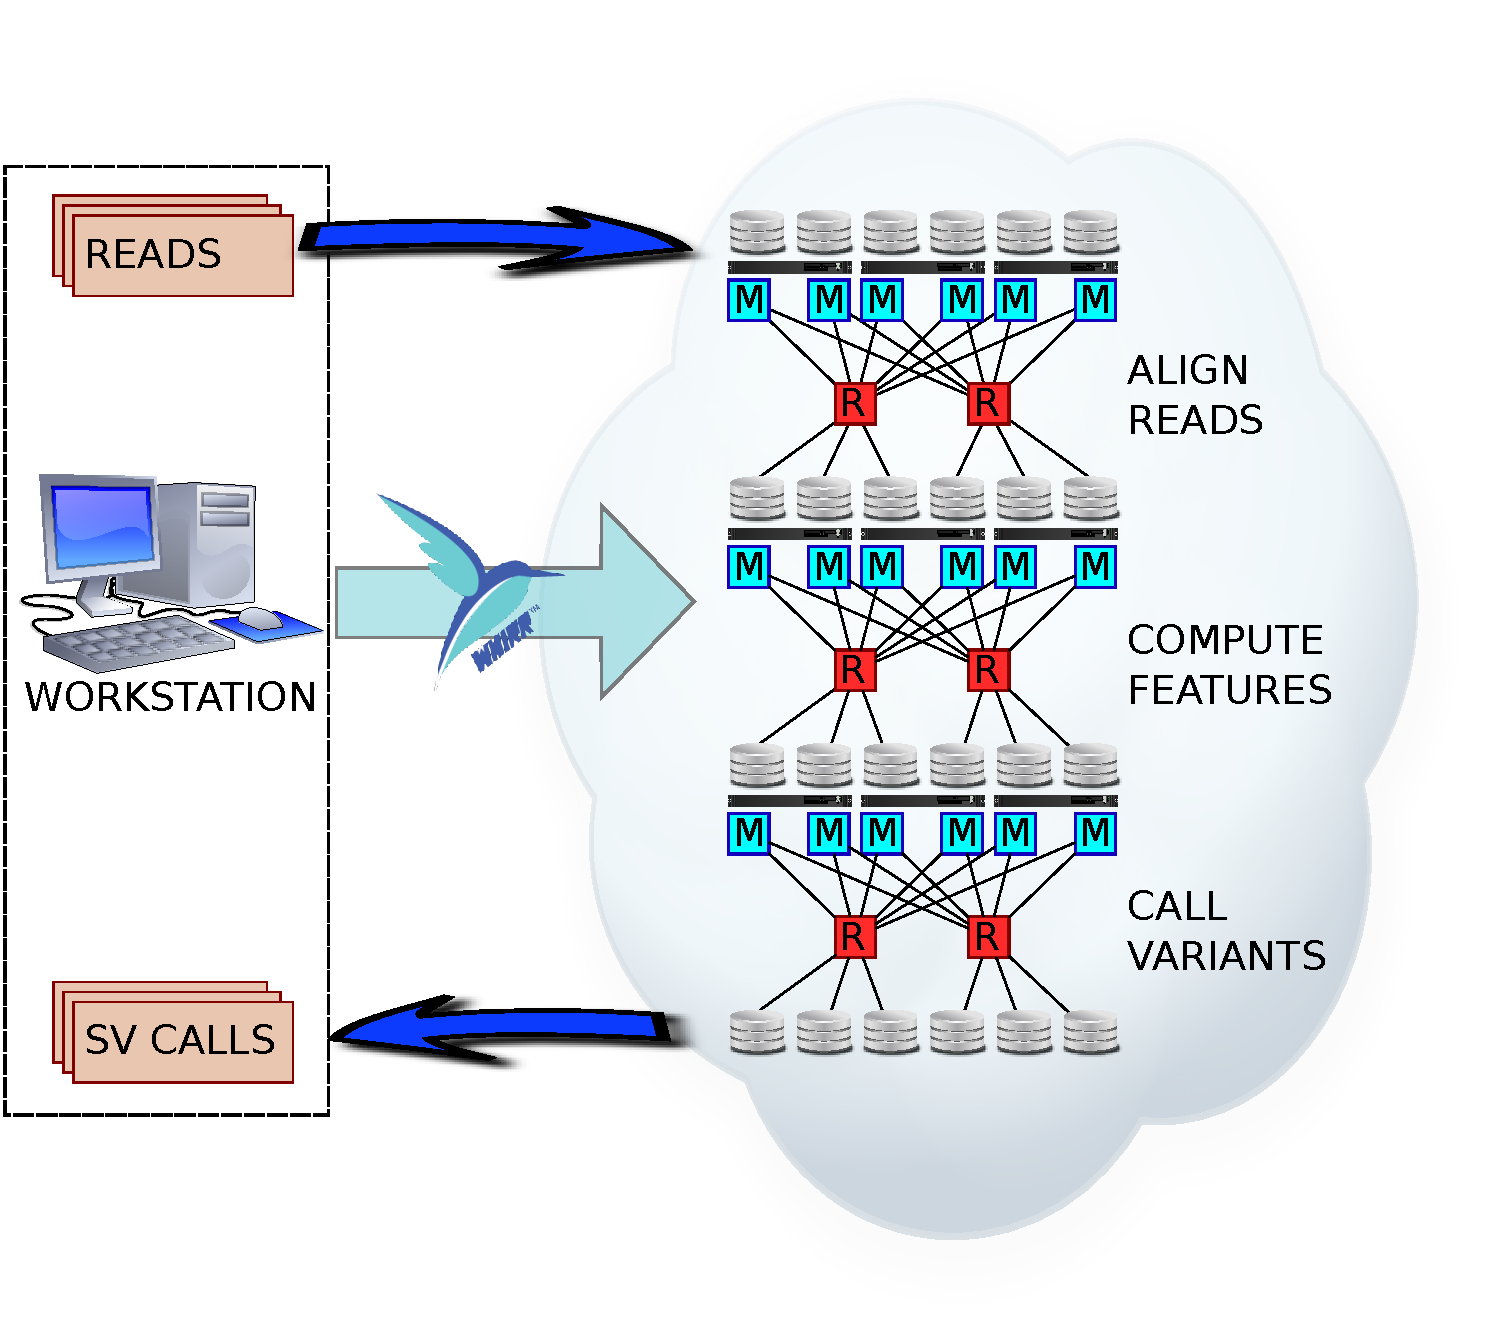
\includegraphics[width=.8\textwidth]{figures/workflow_with_whirr.png}
\caption{An overview of the steps of the MapReduce SV detection workflow. Reads are first uploaded to a Hadoop cluster from local storage. Processing is then then divided into three MapReduce jobs: 1) Mapping with sensitive settings. 2) Computation of features across the genome. 3) Calling structural variations based on the features computed in the previous step. Finally, SV predictions can be downloaded from the Hadoop cluster and examined and annotated. Cloudbreak can also use the Apache Whirr library to automatically provision Hadoop clusters on and deploy data to cloud providers such as Amazon Elastic Compute Cloud.}
\label{cloudbreak_workflow}
\end{figure}


The \textsc{Align Reads} job uses existing alignment tools to discover mapping locations for each read pair. Aligners can be executed to report multiple possible mappings for each read, or only the best possible mapping. Given a set of read pairs, each of which consists of a read pair identifier $rpid$ and two sets of sequence and quality scores $<s,q>$, each mapper aligns each pair end set $<s,q>$ in either single- or paired end mode and emits possible mapping locations under the $rpid$ key. Reducers then collect the alignments for each paired end, making them available under one key for the next job. 

In the \textsc{Compute Features} job, we compute a set of features for each location in the genome. To begin, we tile the genome with small fixed-width, non-overlapping intervals. For the experiments reported in Chapter~\ref{chap_cloudbreak_eval} we use an interval size of 25bp (see Section~\ref{section_window_size} for an exploration of the effects of different window sizes on accuracy and runtime). Let $L = \left\{l_1,l_2,\ldots,l_N\right\}$ be the set of intervals covering the entire genome. Let $R^1 = \left\{r^{1}_{1},r^{1}_{2},\ldots,r^{1}_{M}\right\}$ and $R^2 = \left\{r^{2}_{1},r^{2}_{2},\ldots,r^{2}_{M}\right\}$ be the input set of paired reads. Let $A^1 = \left\{a^{1}_{m,1},a^{1}_{m,2},\ldots,a^{1}_{m,K}\right\}$ and $A^2 = \left\{a^{2}_{m,1},a^{2}_{m,2},\ldots,a^{2}_{m,L}\right\}$ be the set of alignments for the left and right reads from read pair $m$. For any given pair of alignments of the two reads in a read pair, $a^{1}_{m,i}$ and $a^{2}_{m,j}$, let the $\textrm{ReadPairInfo } rpi_{m,i,j}$ be information about the pair relevant to detecting SVs, e.g. the fragment size implied by the alignments and the likelihood that the alignments are correct. We then leave two functions to be implemented depending on the application:
\begin{flalign*}
 \textsc{Loci } :& \langle a^{1}_{m,i},a^{2}_{m,j} \rangle \rightarrow L_m \subseteq L \\
 \Phi :& \left\{\textrm{ReadPairInfo }rpi_{m,i,j}\right\} \rightarrow \mathbb{R}^N \\
\end{flalign*}

The first function, \textsc{Loci}, maps an alignment pair to a set of genomic locations to which it is relevant for SV detection; for example, the set of locations overlapped by the internal insert implied by the read alignments.  We optimize this step by assuming that if there exist concordant mappings for a read pair, defined as those where the two alignments are in the proper orientation and with an insert size within three standard deviations of the expected library insert size, one of them is likely to be correct and therefore we do not consider any discordant alignments of the pair. The second function, $\Phi$, maps a set of ReadPairInfos relevant to a given location to a set of real-valued vectors of features useful for SV detection. 

Finally, the third MapReduce job, \textsc{Call Variants}, is responsible for making SV calls based on the features computed at each genomic location. It calls another application-specific function: 

 \[ \textsc{PostProcess} : \left\{\phi_1,\phi_2,\ldots,\phi_N\right\} \rightarrow \left\{\langle  \textrm{SVType } s, l_{start}, l_{end} \rangle\right\} \]

This function maps the sets of features for related loci into a set of SV calls characterized by their type $s$ (i.e Deletion, Insertion, etc.) and their breakpoint locations $l_{start}$ and $l_{end}$. We parallelize this job in MapReduce by making calls for each chromosome in parallel, which we achieve by associating a location and its set of features to its chromosome in the map phase, and then making SV calls for one chromosome in each reduce task.

\begin{algorithm}
\algrenewcommand\algorithmicprocedure{\textbf{job}}
 \begin{algorithmic}[1]
 \Procedure{Alignment}{}
 \Function{Map}{$\textrm{ReadPairId }rpid, \textrm{ReadId }r, \textrm{ReadSequence }s, \textrm{ReadQuality }q$}
 \ForAll{$ \textrm{Alignments }a \in \textsc{Align}(<s,q>)$}
 \State $\textsc{Emit}(\textrm{ReadPairId }rpid, \textrm{Alignment }a)$
 \EndFor
 \EndFunction
 \Function{Reduce}{$\textrm{ReadPairId }rpid, \textrm{Alignments }a_{1,2,\ldots}$}
 \State $\textrm{AlignmentPairList }ap \gets \textsc{ValidAlignmentPairs}(a_{1,2,\ldots})$
 \State $\textsc{Emit}(\textrm{ReadPairId }rp, \textrm{AlignmentPairList } ap)$
 \EndFunction
 \EndProcedure

 \Procedure{Compute SV Features}{}
 \Function{Map}{$\textrm{ReadPairId }rp, \textrm{AlignmentPairList }ap$}
 \ForAll{$ \textrm{AlignmentPairs }<a_1,a_2> \in ap$}
 \ForAll{$ \textrm{GenomicLocations }l \in \textsc{Loci }(a_1,a_2)$}
 \State $ \textrm{ReadPairInfo }rpi \gets <\textrm{InsertSize}(a_1,a_2), \textrm{AlignmentScore}(a_1,a_2)>$
 \State $\textsc{Emit}(\textrm{GenomicLocation }l, \textrm{ReadPairInfo }rpi)$
 \EndFor
 \EndFor
 \EndFunction
 \Function{Reduce}{$\textrm{GenomicLocation }l, \textrm{ReadPairInfos }rpi_{1,2,\ldots}$}
 \State $\textrm{SVFeatures } \phi_l \gets \Phi(\textrm{InsertSizes }i_{1,2,\ldots}, \textrm{AlignmentScores }q_{1,2,\ldots})$
 \State $\textsc{Emit}(\textrm{GenomicLocation }l, \textrm{SVFeatures } \phi_l)$
 \EndFunction
 \EndProcedure

 \Procedure{Call SVs}{}
 \Function{Map}{$\textrm{GenomicLocation }l, \textrm{SVFeatures } \phi_l$}
 \State $\textsc{Emit}(\textrm{Chromosome}(l), <l,\phi_l>)$
 \EndFunction
 \Function{Reduce}{$\textrm{Chromosome }c, \textrm{GenomicLocation } l_{1,2,\ldots},\phi_{1,2,\ldots}$}
 \State $\textrm{StructuralVariationCalls } svs_c \gets \textsc{PostProcess }(\phi_{1,2,\ldots})$
 \EndFunction
 \EndProcedure
 \end{algorithmic}
\caption{The algorithmic framework for SV calling in MapReduce.}
\label{cb_algo}
\end{algorithm}

\section{Discussion}\label{section_framework_discussion}

The framework that we have just described is agnostic to the type of structural variations that the user wishes to detect. In the next chapter, we describe Cloudbreak, our implementation of this framework that identifies small deletions and insertions. To do so, it defines the relevant information from each pair (the ReadPairInfo) as information about the insert size implied by the mapping of the paired reads, sends them to every location which is spanned by that read pair in the reference genome, and then computes features from them by modeling the expected distribution of insert sizes at each location with a Gaussian Mixture Model. We demonstrate some of the strengths of this particular implementation in Chapter~\ref{chap_cloudbreak_eval}. However, we believe that this general framework could be applied to many other SV detection problems. For example, to detect inversions, one might define a different ReadPairInfo for each pair that includes information about the orientation of the mappings. Translocation detection programs might emit ReadPairInfos that contain information about the chromosomes linked to by interchromosomal mappings, which the $\Phi$ function would then cluster to see if a preponderance of those mappings point to the same breakpoint location. In addition to paired mapping locations, it would also be possible to design ReadPairInfo and feature function definitions that allowed the computation of read depth or split read related features, enabling the integration of more of the signals available in the data set. We will explore one possible way to integrate disparate features such as these in Chapter~\ref{chap_crf}. Use of the Hadoop/MapReduce computing framework would ensure that any of these applications, if carefully designed, could enjoy the benefits of redundancy, data locality, and scalability we described in Section~\ref{section_hadoop_description}, and therefore will be able to grow to meet the rising demands of genomics applications in the near future.